\chapter{Results I --- Bytes, Placement and Loss}\label{ch:bytes}

\needswork{STATUS: DRAFTED. Every number here is reproduced from a committed artifact by an
automated gate; figures are regenerated from frozen data.}

\section{E1 --- authentication dominates after compression}

Thirty seeds of one thousand seeded telemetry records per encoding, inline placement, $\ga = 64$\,B.

\begin{table}[h]
\centering
\caption{Measured record size and authentication fraction. Compression moves the bottleneck.}
\label{tab:e1}
\begin{tabular}{lrrl}
\toprule
encoding & mean bytes & $\varphi$ at $\ga{=}64$ & role \\
\midrule
JSON        & 191.09 & 25.1\% & naive baseline \\
CBOR        & 66.25  & 49.1\% & compression-only baseline \\
MessagePack & 65.16  & 49.6\% & --- \\
\textbf{delta-CBOR} & \textbf{45.00} & \textbf{58.7\%} & the co-design optimum \\
\bottomrule
\end{tabular}
\end{table}

This is \Cref{thm:t1} instantiated: at delta encoding the signature is \emph{larger} than the record
it signs. The motivating claim of the thesis is a measurement, not a conjecture.

\begin{figure}[h]
\centering
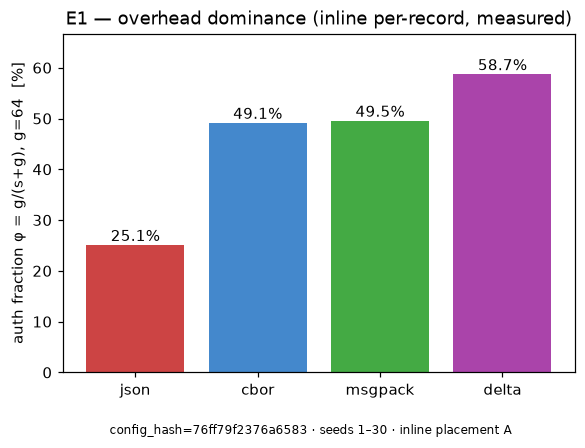
\includegraphics[width=0.7\textwidth]{fig_e1_dominance.png}
\caption{Authentication fraction across encodings. Every byte saved on the payload raises the
fraction spent on cryptography.}
\label{fig:e1}
\end{figure}

\begin{remark}[$s$ is not a property of the encoding alone]
The sizes above are measured over the first $\sim$50 seconds of each simulated flight. Sequence
numbers and timestamps grow with the record index, and variable-length encodings charge for the
extra digits, so JSON, CBOR and MessagePack all grow by 2--4\,B over a ten-times-longer window
while delta-CBOR stays flat --- it encodes differences. The bootstrap interval quoted for CBOR is
$\pm0.02$\,B and describes \emph{seed} variation; the systematic dependence on window length is
$\approx 2.7$\,B, roughly $150\times$ wider. The direction is conservative: a longer flight inflates
the baseline and leaves the optimum alone, so the reported saving is the pessimistic end.
\end{remark}

\section{E2 --- batching is the cure, and which ceiling binds}

Sweeping placement A against B across encodings and MTU budgets confirms \Cref{prop:t2}
qualitatively and \Cref{thm:t2a} quantitatively. At $M = 256$ the MTU binds and amplification is
operative; at $M = 576$ and $M = 1500$ freshness binds and the marginal value of compression is
$1.0000$ to twelve decimal places.

\textbf{The practical consequence.} On 802.11 the amplification law that motivates aggressive
compression is never operative. Compression still pays --- it pays exactly $1\times$.

\begin{figure}[h]
\centering

\includegraphics[width=0.7\textwidth]{fig_e2_batching.png}
\caption{Per-record cost against batch size. The curve flattens where the freshness ceiling takes
over from the frame-size ceiling.}
\label{fig:e2}
\end{figure}

\section{E3 --- the loss frontier}

Measured verifiability against batch size and loss probability, placement B versus D. Frame-level
batching Pareto-dominates block-level for all $V > (1-p)^2$, and at $\varepsilon = p$ block-level is
infeasible beyond one frame, as \Cref{thm:t3} requires.

\begin{remark}[What this experiment does and does not validate]
The emulator implements independent per-frame loss, which is also what the closed form assumes.
Agreement is therefore a \emph{consistency check}, not a validation of the loss model. What rescues
the ordering is \Cref{thm:t3c}, which holds for any stationary loss process, plus Gilbert--Elliott
simulation at matched mean rate showing $V_D$ approaching but never reaching $1-p$.
\end{remark}

\begin{figure}[h]
\centering

\includegraphics[width=0.7\textwidth]{fig_e3_frontier.png}
\caption{The loss-robustness frontier. Block-level authentication trades verifiability for bytes at
a rate the constraint does not permit.}
\label{fig:e3}
\end{figure}
